% \documentclass[11pt]{article}
% \usepackage[margin=4cm]{geometry}
% \usepackage{algpseudocode}
% \usepackage{algorithm}
% \begin{document}

% % If you would like to add line numbers to the algorithm, you can add the first line number to the environment as an optional argument \begin{algorithmic}[1]
% \begin{algorithmic}
% \State $i \gets 10$
% \If{$i\geq 5$} 
%     \State $i \gets i-1$
% \Else
%     \If{$i\leq 3$}
%         \State $i \gets i+2$
%     \EndIf
% \EndIf 
% \end{algorithmic}

% The above algorithm example is not captioned. If you need a captioned algorithm, load the \verb|algorithm| package, and add 
% \begin{verbatim}
% \begin{algorithm}
% \caption{...}
% ...
% \end{algorithm}
% \end{verbatim}
% around your \verb|algorithmic| environment. You can use \verb|\label{...}| after the \verb|\caption| so that the algorithm number can be cross-referenced, e.g.~Algorithm~\ref{alg:cap} and \ref{alg:wordy}.

% \begin{algorithm}[hbt!]
% \caption{An algorithm with caption}\label{alg:cap}
% \begin{algorithmic}
% \Require $n \geq 0$
% \Ensure $y = x^n$
% \State $y \gets 1$
% \State $X \gets x$
% \State $N \gets n$
% \While{$N \neq 0$}
% \If{$N$ is even}
%     \State $X \gets X \times X$
%     \State $N \gets \frac{N}{2} $  \Comment{This is a comment}
% \ElsIf{$N$ is odd}
%     \State $y \gets y \times X$
%     \State $N \gets N - 1$
% \EndIf
% \EndWhile
% \end{algorithmic}
% \end{algorithm}

% The \verb|algorithm| environment is a \emph{float}, like \verb|table| and \verb|figure|, so you can add float placement modifiers \verb|[hbt!]| after \verb|\begin{algorithm}| if necessary.

% \begin{algorithm}[hbt!]
% \caption{Another algorithm with caption}\label{alg:wordy}
% \begin{algorithmic}
% \Require{Write here the required data}
% \Ensure{Write here the expected result}
%  \State initialization;
%  \While{While condition}
%   \State instructions;
%   \If{condition}
%    \State instructions1;
%    \State instructions2;
%   \Else
%    \State instructions3;
%   \EndIf
%  \EndWhile
% \end{algorithmic}
% \end{algorithm}

% The \verb|algorithm| package also provides a \verb|\listofalgorithms| command that works like \verb|\listoffigures|, but for captioned algorithms:

% \listofalgorithms

% \end{document}


\documentclass[
    chapter=TITLE,
    12pt, 		% Tamanho da fonte
    openright,% Capítulos começam em pág. ímpar (insere página vazia caso preciso)
    oneside, 	% Para impressão somente verso. Oposto a impressão em verso e anverso
    hidelinks,
    a4paper, 	% Tamanho do papel
    english, 	% Idioma adicional para hifenização
    brazil 		% o último idioma é o principal do documento
    ]{abntex2}

\renewcommand{\theequation}{\arabic{equation}}  
\usepackage[utf8]{inputenc}
\usepackage{tikz}
\usepackage{wrapfig}
\usetikzlibrary{calc}
\usepackage{lipsum} 	% para geração de dummy text
\usepackage{multirow}
\usepackage{algpseudocode}
\usepackage{algorithm}
\usepackage{svg}

\usepackage{pdflscape} %para poder rotacionar a página
\usepackage[table,xcdraw]{xcolor}

% Pacotes
%% Sumário
\usepackage{tocloft}

%% Referência
\usepackage[hyphenbreaks]{breakurl}
% \usepackage[alf]{abntex2cite}
% \usepackage[alf,abnt-etal-list=0,abnt-etal-cite=3]{abntex2cite} %et al qnd cita apenas
\usepackage[alf,bibjustif,abnt-etal-cite=2]{abntex2cite} %et al na referência tbm e justificada


%\usepackage[hyphenbreaks]{breakurl}
%\usepackage[num,overcite,'-emphasize=em]{abntex2cite}

%% Codificação
\usepackage[T1]{fontenc} 	% Codificação de saída

%% Fonte
\usepackage{times} 			% Times New Roman

\usepackage{lastpage} 		% Usado pela Ficha catalográfica
\usepackage{indentfirst} 	% Indenta o primeiro parágrafo de cada seção.
\usepackage{color} 				% Controle das cores
\usepackage{microtype} 		% Para melhorias de justificação
\usepackage{lscape} 			% Permite a criação de conteúdo em modo paisagem
\usepackage{hyperref} 		% Criação de links
\usepackage{etoolbox}

%% Tabelas
\usepackage{multirow}

%% Equação
\usepackage{amsmath}

%% Sumário
\usepackage{textcase}

%% Imagens
\usepackage{graphicx} % Inclusão de gráficos

%% Tamanho e alinhamento das legendas
\usepackage[
	singlelinecheck=false,
	justification=justified,
	font=footnotesize
	]
	{caption}
\usepackage{pdfpages}
%% Para impressão do Json
\usepackage{minted}


\usepackage{listings}

\renewcommand
	{\familydefault}
	{\sfdefault} 			% Seta fonte default

%% Redefine booleans
%\setboolean{ABNTEXuppersubsection}{false}

%% Cabeçalho padrao
\makepagestyle
	{abntheadings}
\makeevenhead
	{abntheadings}
	{\ABNTEXfontereduzida\thepage}
	{}
	{\ABNTEXfontereduzida\textit\leftmark}
\makeoddhead
	{abntheadings}
	{}
	{}
	{\ABNTEXfontereduzida\thepage}
\makeheadrule
	{abntheadings}
	{0pt}
	{\normalrulethickness}

%% Cabeçalho do inicio do capitulo
\makepagestyle
	{abntchapfirst}
\makeoddhead
	{abntchapfirst}
	{}
	{}
	{\ABNTEXfontereduzida\thepage}


% Estilos
\autor{João Matheus Ramos Gama} 	%Nome do autor
% Especificidades para a entrada de autor pessoal: – sobrenome com indicativo de parentesco
% Quando o autor é brasileiro, trate o grau de parentesco como parte do sobrenome.
% Exemplo: Autor: Luís Fernando Carvalho Neto - Entrada: CARVALHO NETO, L. F.
\newcommand{\entradaAutor}{Ramos Gama, João Matheus} % Sem ponto no final
% Titulo do trabalho
\titulo{Desaprendizado de Máquina: Estabilidade do modelo após o "esquecimento"} %Título do trabalho
\newcommand{\englishTitle}{Medical monitoring and assistance system (MMAS).}
\data{\today}			%Ano de publicação
\local{Nova Friburgo}	%Local
%% Membros da banca
\newcommand{\membrobancaA}{}
\newcommand{\membrobancaB}{}
\newcommand{\membrobancaC}{}

\providecommand
	{\imprimirmembrobancaA}
	{}
\providecommand
	{\imprimirmembrobancaAinst}
	{}
\renewcommand
	{\membrobancaA}
	[2]
	[\imprimirinstituicao]
	{\renewcommand
		{\imprimirmembrobancaA}
		{#2}
		\renewcommand
		{\imprimirmembrobancaAinst}
		{#1}
	}

\providecommand
	{\imprimirmembrobancaB}
	{}
\providecommand
	{\imprimirmembrobancaBinst}
	{}
\renewcommand
	{\membrobancaB}
	[2]
	[\imprimirinstituicao]
	{
		\renewcommand
		{\imprimirmembrobancaB}
		{#2}
		\renewcommand
		{\imprimirmembrobancaBinst}
		{#1}
	}

\providecommand
	{\imprimirmembrobancaC}
	{}
\providecommand
	{\imprimirmembrobancaCinst}
	{}
\renewcommand
	{\membrobancaC}
	[2]
	[\imprimirinstituicao]
	{
		\renewcommand
		{\imprimirmembrobancaC}
		{#2}
		\renewcommand
		{\imprimirmembrobancaCinst}
		{#1}
	}

\newcommand
	{\imprimirmeOrientadorinst}
	{\imprimirinstituicao}
\newcommand
	{\imprimirmeCoorientadorinst}
	{\imprimirinstituicao}

%% Natureza do trabalho
\providecommand{\imprimirnaturezatrabalho}{}
\newcommand{\naturezatrabalho}[1]{
	\renewcommand{\imprimirnaturezatrabalho}{#1}
}

%% Redefinir resumo
\renewenvironment{resumo}[1][\resumoname]{%
	\pretextualchapter{#1}
}{\PRIVATEclearpageifneeded}

%% Redefinir dedicatória
\renewenvironment{dedicatoria}[1][]
{
	\ifthenelse{\equal{#1}{}}{
		\PRIVATEbookmarkthis{\dedicatorianame}
	}{\preamblealchapter{#1}}
	
	\vspace*{\fill}
}
{}

\renewenvironment{epigrafe}[1][]
{
	\ifthenelse{\equal{#1}{}}{
		\PRIVATEbookmarkthis{\epigraphname}
	}{\pretextualchapter{#1}}
	
	\vspace*{\fill}
}
{
	
}

%% Comando para inserir sigla
\newcommand{\sigla}[2][]{
	\item[#1] \textit{#2}
}


%% Comando para inserir simbolo
\newcommand{\simbolo}[2][]{
	\item[#1] \textit{#2}
}
%% Redefinição da formatação do \chapter
\renewcommand{\ABNTEXchapterfont}{\normalfont\fontseries{b}\selectfont}
\renewcommand{\ABNTEXchapterfontsize}{\normalsize}
\renewcommand{\ABNTEXpartfont}{\fontseries{b}\selectfont\selectfont}
\renewcommand{\ABNTEXpartfontsize}{\normalsize}
\renewcommand{\ABNTEXsectionfont}{\normalfont\selectfont} %\fontseries{b}
\renewcommand{\ABNTEXsectionfontsize}{\normalsize}
\renewcommand{\ABNTEXsubsectionfont}{\normalfont}
\renewcommand{\ABNTEXsubsectionfontsize}{\normalsize}
\renewcommand{\ABNTEXsubsubsectionfont}{\normalfont}
\renewcommand{\ABNTEXsubsubsectionfontsize}{\normalsize}
\renewcommand{\ABNTEXsubsubsubsectionfont}{\normalfont}
\renewcommand{\ABNTEXsubsubsubsectionfontsize}{\normalsize}
%\renewcommand{\ABNTEXsubsubsectionfont}{\normalfont\fontseries{b}\selectfont}
%\renewcommand{\ABNTEXsubsubsectionfontsize}{\normalsize}
%\renewcommand{\ABNTEXsubsubsubsectionfont}{\normalfont\itshape\selectfont}
%\renewcommand{\ABNTEXsubsubsubsectionfontsize}{\normalsize}



%% Redefinição da formatação de Parágrafos 
\setlength{\parindent}{1.3cm}
\setlength{\parskip}{0cm}



%% Sumário
\makeatletter
\addtocontents{toc}{%
	\protect\renewcommand{\protect\cftchapterleader}{%-- switch it on here
		\normalsize\normalfont\protect\cftdotfill{\protect\cftdotsep}}}
\renewcommand{\cftchapterpresnum}{\normalfont} % Numeração do capítulo não ficar em negrito
\renewcommand{\cftchapterpagefont}{\normalfont} % Páginas do capítulo não ficar em negrito
\renewcommand*{\cftchapterfont}{\normalfont\bfseries} % Título do capítulo em negrito
\renewcommand{\chapnumfont}{\normalfont\normalsize}
\renewcommand*{\cftsectionfont}{\normalfont} %\fontseries{b}
\renewcommand*{\cftsubsectionfont}{\normalfont}
\renewcommand*{\cftsubsubsectionfont}{\normalfont}
\renewcommand*{\cftsubsubsubsectionfont}{\normalfont}
\renewcommand*{\cftparagraphfont}{\normalfont} %\itshape



%% Forca underline na secao terciaria
\newcommand{\tmpsubsection}[1]{}
\let\tmpsubsection=\subsection
\renewcommand{\subsection}[1]{\tmpsubsection{\underline{#1}}}

%% Forca underline na secao secundaroa
\newcommand{\tmpsection}[1]{}
\let\tmpsection=\section
\renewcommand{\section}[1]{\tmpsection{\textbf{#1}}}
\makeatother
%% Tornar as seções secundários com fonte em maiúscula
%\makeatletter
%\let\oldcontentsline\contentsline
%\def\contentsline#1#2{%
%  \expandafter\ifx\csname l@#1\endcsname\l@section
%    \expandafter\@firstoftwo
%  \else
%    \expandafter\@secondoftwo
%  \fi
%  {%
%    \oldcontentsline{#1}{\MakeTextUppercase{#2}}%
%  }{%
%    \oldcontentsline{#1}{#2}%
%  }%
%}
%\makeatother

%% Tornar a entrada "Referências" com fonte em maiúscula
%%\addto\captionsbrazil{
%%    \renewcommand{\bibname}{REFER\^ENCIAS}
%%}
% Legendas
\makeatletter
\patchcmd{\caption@@@make}
{\ifcaption@star}
{\ifcaption@star\small}
{}{}
\makeatother


\graphicspath{ {figures/} }

\preambulo{
Trabalho de conclusão de curso apresentado como pré-requisito para obtenção do título de Engenheiro de Computação, ao Departamento de Modelagem Computacional, do Instituto Politécnico, da Universidade do Estado do Rio de Janeiro.
}

\orientador{Prof. Dr. Roberto Pinheiro Domingos }
\tipotrabalho{monografia}		%Define as configurações do arquivo

\begin{document}
    \newpage
\pagenumbering{arabic}
	%Capa
	\renewcommand{\imprimircapa}{%
	\begin{center}
		\begin{tikzpicture}[remember picture, overlay]
		\draw[line width = 4pt] ($(current page.north west) + (20mm, -20mm)$) rectangle ($(current page.south east) + (-10mm,10mm)$);
		\draw[line width = 1pt] ($(current page.north west) + (21.5mm,-21.5mm)$) rectangle ($(current page.south east) + (-11.5mm,11.5mm)$);
		\end{tikzpicture}
		\begin{capa}
			\begin{minipage}[r]{0.1\linewidth}
				
\includegraphics[width=1.5\linewidth]{uerj}
            \end{minipage}%
            \begin{minipage}[c]{0.7\linewidth}
				\begin{center}
					\textbf{UNIVERSIDADE DO ESTADO DO \\ RIO DE JANEIRO}\\
					\noindent\rule{7cm}{0.4pt}\\
					\textbf{INSTITUTO POLITÉCNICO \\ GRADUAÇÃO EM ENGENHARIA \\DE COMPUTAÇÃO}\\
				\end{center}
			\end{minipage}%
   			\begin{minipage}[r]{0.1\linewidth}
				
\includegraphics[width=1.5\linewidth]{iprj}
            \end{minipage}%		
			\vspace*{4.5cm}
			\center
			\textbf{\large\imprimirautor}
			\vspace*{3cm}
			\begin{center}
				\textbf{\large\imprimirtitulo}
			\end{center}
			\vfill
			\textbf{
				\large\imprimirlocal
				\\	
				\large \the\year
			}
			\vspace*{1cm}
		\end{capa}
	\end{center}
}
\imprimircapa
	
	%Folha de rosto
	\makeatletter
\renewcommand{\folhaderostocontent}{
	\begin{center}
		\begin{tikzpicture}[remember picture, overlay]
		\draw[line width = 4pt] ($(current page.north west) + (20mm, -20mm)$) rectangle ($(current page.south east) + (-10mm,10mm)$);
		\draw[line width = 1pt] ($(current page.north west) + (21.5mm,-21.5mm)$) rectangle ($(current page.south east) + (-11.5mm,11.5mm)$);
		\end{tikzpicture}
		
		\begin{minipage}[r]{0.1\linewidth}
			
\includegraphics[width=1.5\linewidth]{uerj} 
		\end{minipage}%
		\begin{minipage}[c]{0.7\linewidth}
			\begin{center}
				\textbf{UNIVERSIDADE DO ESTADO DO \\ RIO DE JANEIRO}\\
				\noindent\rule{7cm}{0.4pt}\\
				\textbf{INSTITUTO POLITÉCNICO \\ GRADUAÇÃO EM ENGENHARIA \\DE COMPUTAÇÃO}\\
			\end{center}
		\end{minipage}%
		\begin{minipage}[c]{0.1\linewidth}
			
\includegraphics[width=1.5\linewidth]{iprj} 
		\end{minipage}
		\vspace*{2cm}
		\begin{center}
			{\large\imprimirautor}
			\vspace*{\fill}\vspace*{\fill}
			\begin{center}
				\textbf{\large\imprimirtitulo}
			\end{center}
			\vspace*{\fill}
			\abntex@ifnotempty{\imprimirpreambulo}{%
				\hspace{.45\textwidth}
				\begin{minipage}{.5\textwidth}
					\SingleSpacing
					\imprimirpreambulo
				\end{minipage}%
				\vspace*{2cm}
				\vspace*{\fill}
			}%
			{\abntex@ifnotempty{\imprimirinstituicao}{\imprimirinstituicao
					\vspace*{\fill}}}
\begin{flushleft}
{\large\imprimirorientadorRotulo~\imprimirorientador\par}
\end{flushleft}
			\abntex@ifnotempty{\imprimircoorientador}{%
			{\large\imprimircoorientadorRotulo~\imprimircoorientador}%
			}%
            
			\vspace*{\fill}
			{\large\imprimirlocal}
			\par
			{\large\the\year}
			\vspace*{1cm}
		\end{center}	
	\end{center}
}
\makeatother
	\imprimirfolhaderosto

	%Catalogação Biblioteca
	\newcommand{\imprimircatalogacao}{%
	\noindent
	UNIVERSIDADE DO ESTADO DO RIO DE JANEIRO\\
	INSTITUTO POLITÉCNICO \\ 
    CURSO DE ENGENHARIA DE COMPUTAÇÃO\\
	
    \noindent
	Reitora: Gulnar Azevedo e Silva\\
    Vice-reitor: Bruno Rêgo Deusdará Rodrigues \\
	Diretor do Instituto Politécnico: Lucas Venâncio Pires de Carvalho Lima\\
	Coordenador de Curso: Rodrigo Lamblet Mafort\\
	
	\noindent
	Banca Avaliadora Composta por: \imprimirorientador~(Orientador)\\
	\hspace*{6.3cm}Prof. Dr. Nome do professor da banca\\
	\hspace*{6.3cm}Prof. Dr. Nome do professor da banca
	\\
    \\
	% \noindent
   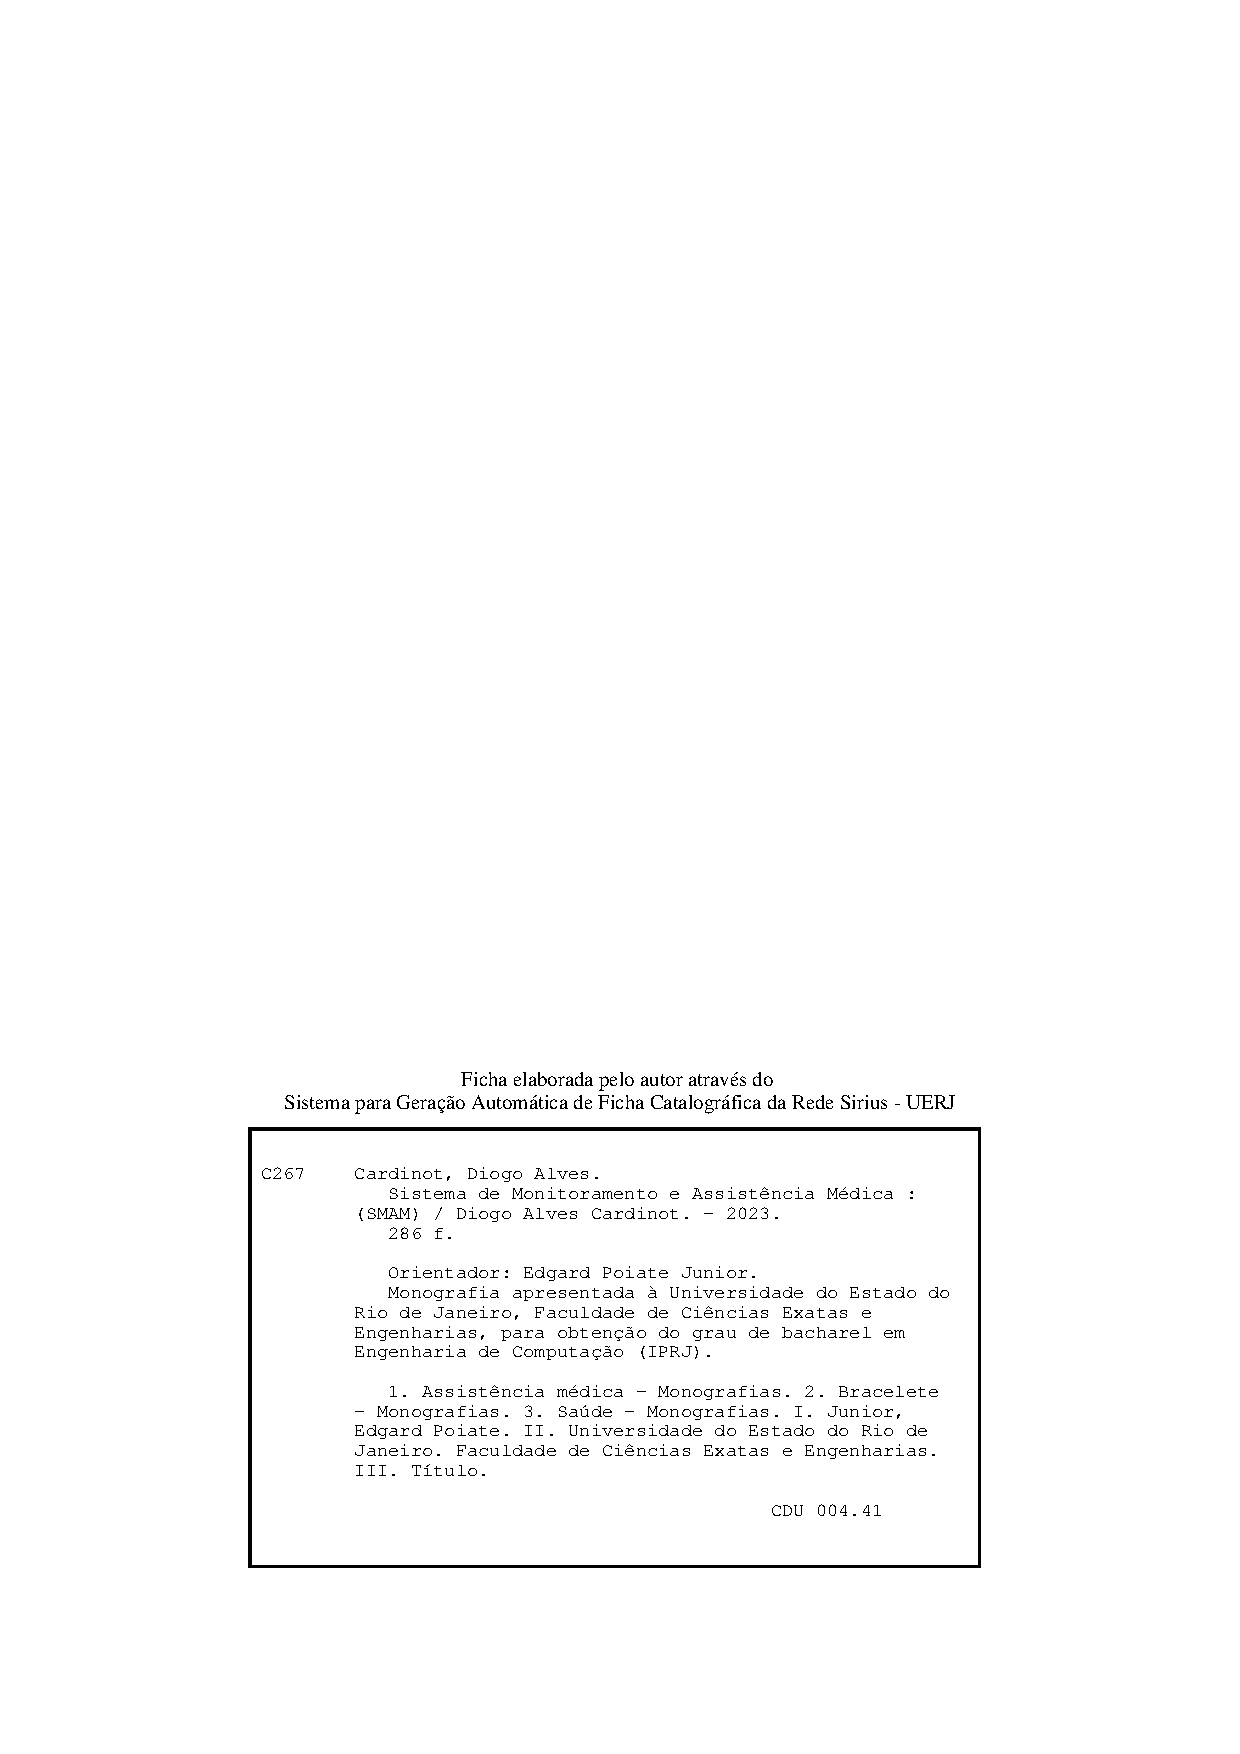
\includegraphics[
        page=1,
        trim={4cm 3cm 0cm 18cm},
	    clip,
	    width={17cm},
        height = {9cm}  %era 10
  ]{fichaBibli.pdf}
  %https://www.rsirius.uerj.br/servicos/elaboracao_ficha/instrucoes   gerar a sua
  %http://www.sirius.uerj.br/ficha/ficha104.php  preencher os dados

	%Endereço: UERJ - IPRJ,  Rua Bonfim, 25 - Prédio 5, Vila Amélia. CEP 28625-570 - Nova Friburgo - RJ - Brasil.\\
\noindent
Endereço: UERJ - IPRJ \\
\hspace*{2cm} CEP 28625-570 - Nova Friburgo - RJ - Brasil.\\

	\noindent
 Este trabalho nos termos da legislação que resguarda os direitos autorais é considerado de propriedade da Universidade do Estado do Rio de Janeiro (UERJ). É permitida a transcrição parcial de partes do trabalho, ou mencioná-lo, para comentários e citações, desde que sem propósitos comerciais e que seja feita a referência bibliográfica completa.
	\begin{flushright}
		\assinatura{\imprimirautor}
	\end{flushright}
}

\imprimircatalogacao
	
	%Folha de aprovação
	\newcommand{\imprimirfolhaaprovacao}{%
	\begin{folhadeaprovacao}
		\begin{center}
			%{\large{\imprimirautor}}\\[1cm]
            {\imprimirautor}\\[1cm]
			\vspace{2cm}
			%{\Large\bfseries\imprimirtitulo}
            {\bfseries\imprimirtitulo}
		\end{center}		
		\vspace{1cm}
		\hspace{.45\textwidth}
		\begin{minipage}{.5\textwidth}
			{\fontsize{12}{12}\selectfont{\imprimirpreambulo}}
		\end{minipage}%
		\\\\\\\\
		\vspace{1cm}
		Aprovado em <dia> de <mês> de <ano>.\\
		\vspace{1.5cm}
		Banca examinadora:
		
		\assinatura{
        \flushleft{\imprimirorientador
        \vspace{}\\Instituto Politécnico - UERJ}}
		   \assinatura{\flushleft{Prof. Dr. Nome do professor da banca\\Instituto Politécnico - UERJ}}
		 \assinatura{\flushleft{Prof. Dr. Nome do professor da banca\\Instituto Politécnico - UERJ}}
		\begin{center}
			\vfill
			%{\large\imprimirlocal}
            {\imprimirlocal}
            \vspace{0.2cm}
			\par
			%{\large\the\year}
            {\the\year}
		\end{center}
		
	\end{folhadeaprovacao}
}

\imprimirfolhaaprovacao

	  %% Elemento opcional (Figura 10).
%% A palavra DEDICATÓRIA deve ser grafada em fonte 12, em
%% maiúsculas, negritada e centralizada na parte superior da folha.
%% O texto da dedicatória deve estar localizado na parte inferior da
%% folha, seguindo as regras gerais de apresentação gráfica.

\begin{epigrafe}[Dedicatória]

<Elemento opcional> Dedico este trabalho a ...

\end{epigrafe}
	%% A palavra AGRADECIMENTOS deve ser grafada em fonte 12,
%% em maiúsculas, negritada e centralizada na parte superior da folha.
%% O texto dos agradecimentos deve ser separado do título por duas
%% linhas em branco com espaçamento 1,5 e digitado de acordo as regras
%% gerais de apresentação gráfica.
%% Se houver necessidade, o texto pode continuar nas folhas seguin-
%% tes, sem incluir a palavra Agradecimentos.

\begin{agradecimentos}

<Elemento opcional> Agradeço primeiramente a ....

\end{agradecimentos}
	  %% Elemento opcional.
%% É uma citação sem aspas – em fonte 12, estilo normal, com es-
%% paço 1,5 – seguida da indicação de autoria, grafada em fonte 12 e em
%% itálico.
%% O texto deve estar localizado no terço inferior da folha, com o ali-
%% nhamento livre, necessário à epígrafe.

\begin{epigrafe}

%\noindent
\flushright{Epígrafe - citação opcional}

\end{epigrafe}
	%% 3.1.9 Resumo em língua portuguesa
%% Elemento obrigatório (Figura 14).
%% Consiste na apresentação sucinta dos pontos relevantes do texto,
%% em um único parágrafo. O resumo deve conter entre 150 e 500 pala-
%% vras e fornecer uma visão rápida e clara dos objetivos, da metodologia,
%% dos resultados e das conclusões do trabalho. Na elaboração do resumo,
%% deve-se usar o verbo na voz ativa, na terceira pessoa do singular.

%% Fonte -> TNR ou Arial, corpo 12.
%% A palavra RESUMO deve aparecer em letras maiúsculas
%% e em negrito.
%% O uso de itálico é permitido em palavras estrangeiras.
%% O uso de letras maiúsculas nas palavras-chave
%% restringe-se ao início da palavra, em nomes próprios
%% e siglas, se for o caso.

%% Alinhamento -> A palavra RESUMO deve estar localizada na margem
%% superior da folha e centralizada, e a referência, alinhada
%% à margem esquerda;
%% O alinhamento é justificado para o texto do resumo,
%% que inicia com parágrafo, e para as palavras-chave.

%% Espaçamento -> A palavra RESUMO deve ser separada da referência por
%% duas linhas em branco de 1,5;
%% Espaço 1 na referência e no resumo e, nas palavras-
%% chave, espaço 1,5.

%% Formato do papel,
%% orientação e margens -> Conforme especificado na seção 1.1.

%% Pontuação -> As palavras-chave devem ser separadas por ponto e
%% terminadas por ponto.

\begin{resumo}
\begin{SingleSpace}

\noindent
\begin{flushleft}
\entradaAutor{}. \textit{\imprimirtitulo}. \the\year. \pageref{LastPage} f. Trabalho de Conclusão de Curso (Graduação em Engenharia de Computação) - Instituto Politécnico, Universidade do Estado do Rio de Janeiro, Nova Friburgo, \the\year.
\end{flushleft}
\vspace{\onelineskip}

\setlength{\parindent}{1.3cm}

\textit{Consiste na apresentação sucinta dos \textbf{pontos relevantes} do texto, em um único parágrafo. O resumo deve conter\textbf{ entre 150 e 500 palavras} e fornecer uma\textbf{ visão rápida e clara dos objetivos}, da metodologia, dos resultados e das conclusões do trabalho. Na elaboração do resumo, deve-se usar o \textbf{verbo na voz ativa}, na terceira pessoa do singular.>
}

\vspace{0.5cm}
O envelhecimento da população no Brasil gera desafios de saúde, incluindo aumento do Alzheimer e risco de fraturas por quedas, afetando a taxa de mortalidade dos idosos. A detecção de crises epilépticas é crucial, dada a falta de consciência dos pacientes, dificultando o ajuste adequado da medicação. A identificação de ocorrências como quedas, ataques epilépticos e parâmetros físicos do usuário é crucial para ajustes no tratamento. Além disso, localizar os usuários também é essencial. \textbf{Nesse contexto}, com o objetivo de reduzir as sequelas causadas após quedas, principalmente em idosos, um sistema de monitoramento e assistência médica torna-se fundamental para abordar esses desafios e melhorar a qualidade de vida da população.  \textbf{Neste projeto}, foi desenvolvido um protótipo que consiste na criação de um sistema ......\textbf{Para atingir esses objetivos, foi desenvolvido} este projeto no qual foi utilizado o microcontrolador ESP32, associado a um acelerometro, um oximetro e medidor de batimentos cardiacos, e um módulo GPS. Os software referente a montagem foi todo desenvolvido dentro da plataforma Arduino IDE, enquanto que a parte refente ao setup foi desenvolvida na linguagem PHP. O protótipo foi validado e o \textbf{resultado geral do projeto} foi satisfatório, pois algumas melhorias em relação a medição da pressão arterial e temperatura corporal.
 

\vspace{\onelineskip}
\noindent Palavras-chave:  assistência médica; bracelete; ESP32; PHP; saúde; XAMPP.

\end{SingleSpace}
\end{resumo}
	%% Elemento obrigatório (Figura 15).
%% Consiste em uma tradução do resumo em português para uma
%% língua estrangeira (em inglês, ABSTRACT; em espanhol, RESUMEN;
%% em francês, RÉSUMÉ), em um único parágrafo, seguido das palavras-
%% -chave representativas do conteúdo do trabalho, na língua estrangeira
%% escolhida.
%% O resumo em outra língua também é precedido pela referência
%% do trabalho, substituindo-se o título em português pelo título na língua
%% estrangeira adotada.
%% No caso de teses, é possível incluir dois resumos em língua es-
%% trangeira.
%% A apresentação gráfica e a ordem dos elementos seguem a mes-
%% ma orientação do resumo em português.

\begin{resumo}[Abstract]
\begin{otherlanguage*}{english}
\begin{SingleSpace}

\noindent
\begin{flushleft}
\entradaAutor{}. \textit{\englishTitle{}} 2023.\pageref{LastPage} f. Trabalho de Conclusão de Curso (Graduação em Engenharia de Computação) - Instituto Politécnico, Universidade do Estado do Rio de Janeiro, Nova Friburgo, 2023.
\end{flushleft}
\vspace{\onelineskip}

\setlength{\parindent}{1.3cm}

The aging population in Brazil poses health challenges, including an increase in Alzheimer's cases and the risk of fractures from falls, impacting the mortality rate of the elderly. Detecting epileptic seizures is crucial due to patients' lack of awareness, complicating the proper adjustment of medication. Identifying incidents such as falls, epileptic attacks, and the user's physical parameters is vital for treatment adjustments. Additionally, user location is essential. In this context, aiming to reduce the consequences of falls, particularly in the elderly, a monitoring and medical assistance system becomes crucial to address these challenges and improve the population's quality of life. In this project, a prototype was developed, creating a real-time monitoring system for patients. The system sends alerts to trusted individuals about falls, the patient's status (conscious and immobile or unconscious and immobile), possible epileptic seizures, and assists in locating patients with Alzheimer's who may be lost. Moreover, the prototype measures the patient's physical parameters and alerts about potential abnormalities. To achieve these objectives, this project utilized the ESP32 microcontroller, coupled with an accelerometer, pulse oximeter, heart rate monitor, and a GPS module. The assembly software was developed within the Arduino IDE platform, while the setup part was implemented in the PHP language. The prototype was validated, and the overall project results were satisfactory, with some improvements needed for blood pressure and body temperature measurements.

\vspace{\onelineskip}
\noindent Keywords: medical care; bracelet; ESP32; health; XAMPP.

\end{SingleSpace}
\end{otherlanguage*}
\end{resumo}
	
	%Lista de Figuras
	\renewcommand*\listfigurename{Lista de Figuras}
	\listoffigures*
	\cleardoublepage

 	%Lista de Tabelas
	\renewcommand*\listtablename{Lista de Tabelas}
	\listoftables*
	\cleardoublepage
 
 % \cleardoublepage
	%\include{abreviaturas}
	\begin{siglas}
\item[AVC] Acidente Vascular Cerebral
\item[CI] Consciente e Imóvel
\item[DA] Doença de Alzheimer
\item [ECG] Eletrocardiograma

\textit{<e outras>}
\\
\\
<OPCIONAL - LISTA EM ORDEM ALFABÉTICA>
\end{siglas}
	\begin{simbolos}
\item[>] Maior que
\item[<] Menor que

\textit{<e outras>}
\\
\\
<OPCIONAL - NA ORDEM EM QUE APARECEM NO TEXTO>
\end{simbolos}
	
	%Sumário
	\pdfbookmark[0]{\contentsname}{toc}
	\tableofcontents*
	\cleardoublepage
	
	 % Elementos textuais
	\textual
	% Workaround para criação de capítulo não-numerado alinhado à margem
\chapter*{}
\noindent
\phantomsection{\MakeUppercase{\textbf{Introdução}}}
\addcontentsline{toc}{chapter}{INTRODUÇÃO}

% \newline
% \newline

%\section{Motivação}

%% FIXME: Adicionar referências
\vspace{1.4cm}

apresentar sobre o desamprendizado de maquina

falar que sabemos as informaçoes que entram mas nao temos ciencia de como ela é tratada no treinamento

falar que nao é totalmente claro quais informações entram devido a grande quantidade

falar sobre o perigo de usar dados com informaçoes criticas a segurança no treinamento

falar sobre os modelos que salvam o contexto da conversa podendo salvar informações sobre dados sensiveis


\vspace{0.5cm}

\textit{< Apresentar
o problema investigado e indicar sua origem e relevância (sua importância teórica e/ou prática),\textbf{ situando o leitor no contexto da pesquisa realizada}.
Uma rápida referência a trabalhos anteriores (informações sobre os antecedentes do estudo) dedicados ao problema fornecerá elementos para justificar a realização do próprio trabalho. Na introdução, o autor indicará o \textbf{objetivo geral }do estudo e os \textbf{objetivos específicos} a ele relacionados ou a designação das hipóteses de trabalho.
Espera-se que sejam feitas referências às possibilidades de \textbf{contribuição} do estudo desenvolvido, sem, no entanto, antecipar soluções ou conclusões a que se chegou no trabalho.
>
}
\vspace{0.5cm}
\par No Brasil, atualmente, aproximadamente 15,1\% da população é constituída por indivíduos idosos, que abrangem a população com idade igual ou superior a 60 anos. É previsto que até o ano de 2050, os idosos representarão cerca de 30\% da população do país (\citeauthoronline{IdososBrasil},\citeyear{IdososBrasil}). 

O processo de envelhecimento é um dos principais fatores de risco para o desenvolvimento da doença de Alzheimer (\citeauthoronline{AlzheimerAssociation},\citeyear{AlzheimerAssociation}).  
Além disso, os idosos apresentam maior suscetibilidade a fraturas, muitas das quais afetam áreas que têm um impacto significativo em sua mobilidade (\citeauthoronline{PreventionFalls},\citeyear{PreventionFalls}). 

Entre os fatores críticos que contribuem para essas fraturas, destacam-se as quedas. Além das fraturas, as quedas representam um risco considerável para o desenvolvimento de hemorragias cerebrais, lesões viscerais traumáticas, limitações funcionais e um aumento na taxa de mortalidade. Isso ocorre porque um paciente que sofre uma queda pode perder a consciência e sofrer uma perda significativa de sangue, o que, em última instância, pode resultar em óbito (\citeauthoronline{PreventionFalls}, \citeyear{PreventionFalls}).

É importante salientar que a identificação de situações críticas, como ataques cardíacos, baixa oxigenação no sangue e temperaturas corporais anormais, também é fundamental. Esses eventos podem ocorrer em pacientes idosos, aumentando ainda mais os riscos à saúde. 

Além disso, em relação a outras condições médicas, a epilepsia, uma doença que afeta principalmente crianças e idosos, é uma preocupação significativa no Brasil, com cerca de 3 milhões de pacientes afetados por seus sintomas. 

Como meio de monitorar vários parâmetros de saúde do paciente, como frequência cardíaca, qualidade do sono e atividade física, existem disponíveis nos dispositivos capazes de realizarem tais monitoramentos. 

Considerando a possibilidade de interpretação dos dados apresentados e suas potenciais implicações para os pacientes, surge a ideia de desenvolver um Sistema ....

Essa abordagem busca proporcionar uma possível contribuição ...

\vspace{0.5cm}
\textbf{Organização do trabalho}

\vspace{0.5cm}
<\textbf{Ao final} da introdução, faz-se a \textbf{apresentação dos capítulos que constituem o corpo do trabalho, justificando-os
brevemente}.>

% Considerando os dados apresentados e suas implicações para os pacientes, surge a ideia de desenvolver um Sistema de Monitoramento e Assistência Médica (SMAM). Esse sistema tem como objetivo analisar dados e verificar condições indicativas  não apenas a possível ocorrência de quedas de pacientes, mas também condições indicativas da ocorrência de ataque epilético assim como outros eventos críticos, como ataques cardíacos, níveis baixos de oxigenação no sangue e variações anormais de temperatura corporal.

% Além disso, a capacidade de avaliar a condição do paciente imediatamente após uma queda é de extrema importância para permitir uma resposta rápida e, assim, prevenir possíveis consequências graves, incluindo o óbito. Adicionalmente, o SMAM visa também a identificação de eventos como acidentes vasculares cerebrais (AVC) e labirintite, ampliando sua abrangência na detecção de condições médicas críticas.

% Isso proporciona uma abordagem abrangente e proativa na promoção da saúde e segurança dos pacientes, contribuindo significativamente para a qualidade do atendimento médico.



\vspace{10mm} %5mm vertical space


	\chapter{REVISÃO BIBLIOGRÁFICA}
\label{cap1Revisao}
\textit{< É, de forma geral, a \textbf{revisão das pesquisas} \textbf{e das discussões de outros autores sobre o tema} que será abordado em seu trabalho. Ou seja: é a contribuição das teorias de outros autores para a sua pesquisa. >}


	\chapter{FUNDAMENTAÇÃO TEÓRICA}

\textit{< Apresentar os conceitos estudados para desenvolver o trabalho >}

\section{Métodos de Newton}

\subsection{Método 1}

	\chapter{MATERIAL E MÉTODOS}\label{cap3MatMet}

\textit{
< O desenvolvimento é a parte nuclear do trabalho, por vezes denominada
corpo do trabalho. Nessa parte, discute-se o problema apresentado
na introdução, bem como aspectos da metodologia utilizada para
a realização do estudo.
De acordo com as características do problema, das técnicas utilizadas
e do estilo do autor, pode-se dividir o desenvolvimento em partes
ou capítulos, e cada capítulo em subtítulos ou itens, sem que se perca a
unidade do trabalho. >
}

\vspace{0.5cm}
Este capítulo aborda as etapas do desenvolvimento do projeto, os materiais utilizados e a metodologia.

\section{Materiais}

\section{Metodologia}


	\chapter{RESULTADOS E DISCUSSÃO}


Neste capítulo, são expostos todos os resultados alcançados até o momento ao longo do progresso do projeto, abrangendo ...

A montagem do protótipo pode ser vista na Figura \ref{fig:prototipo2}. 

\begin{figure}[H]
    \centering
    \captionsetup{justification=centering}
    \caption{Montagem física do protótipo vista em diagonal} 
    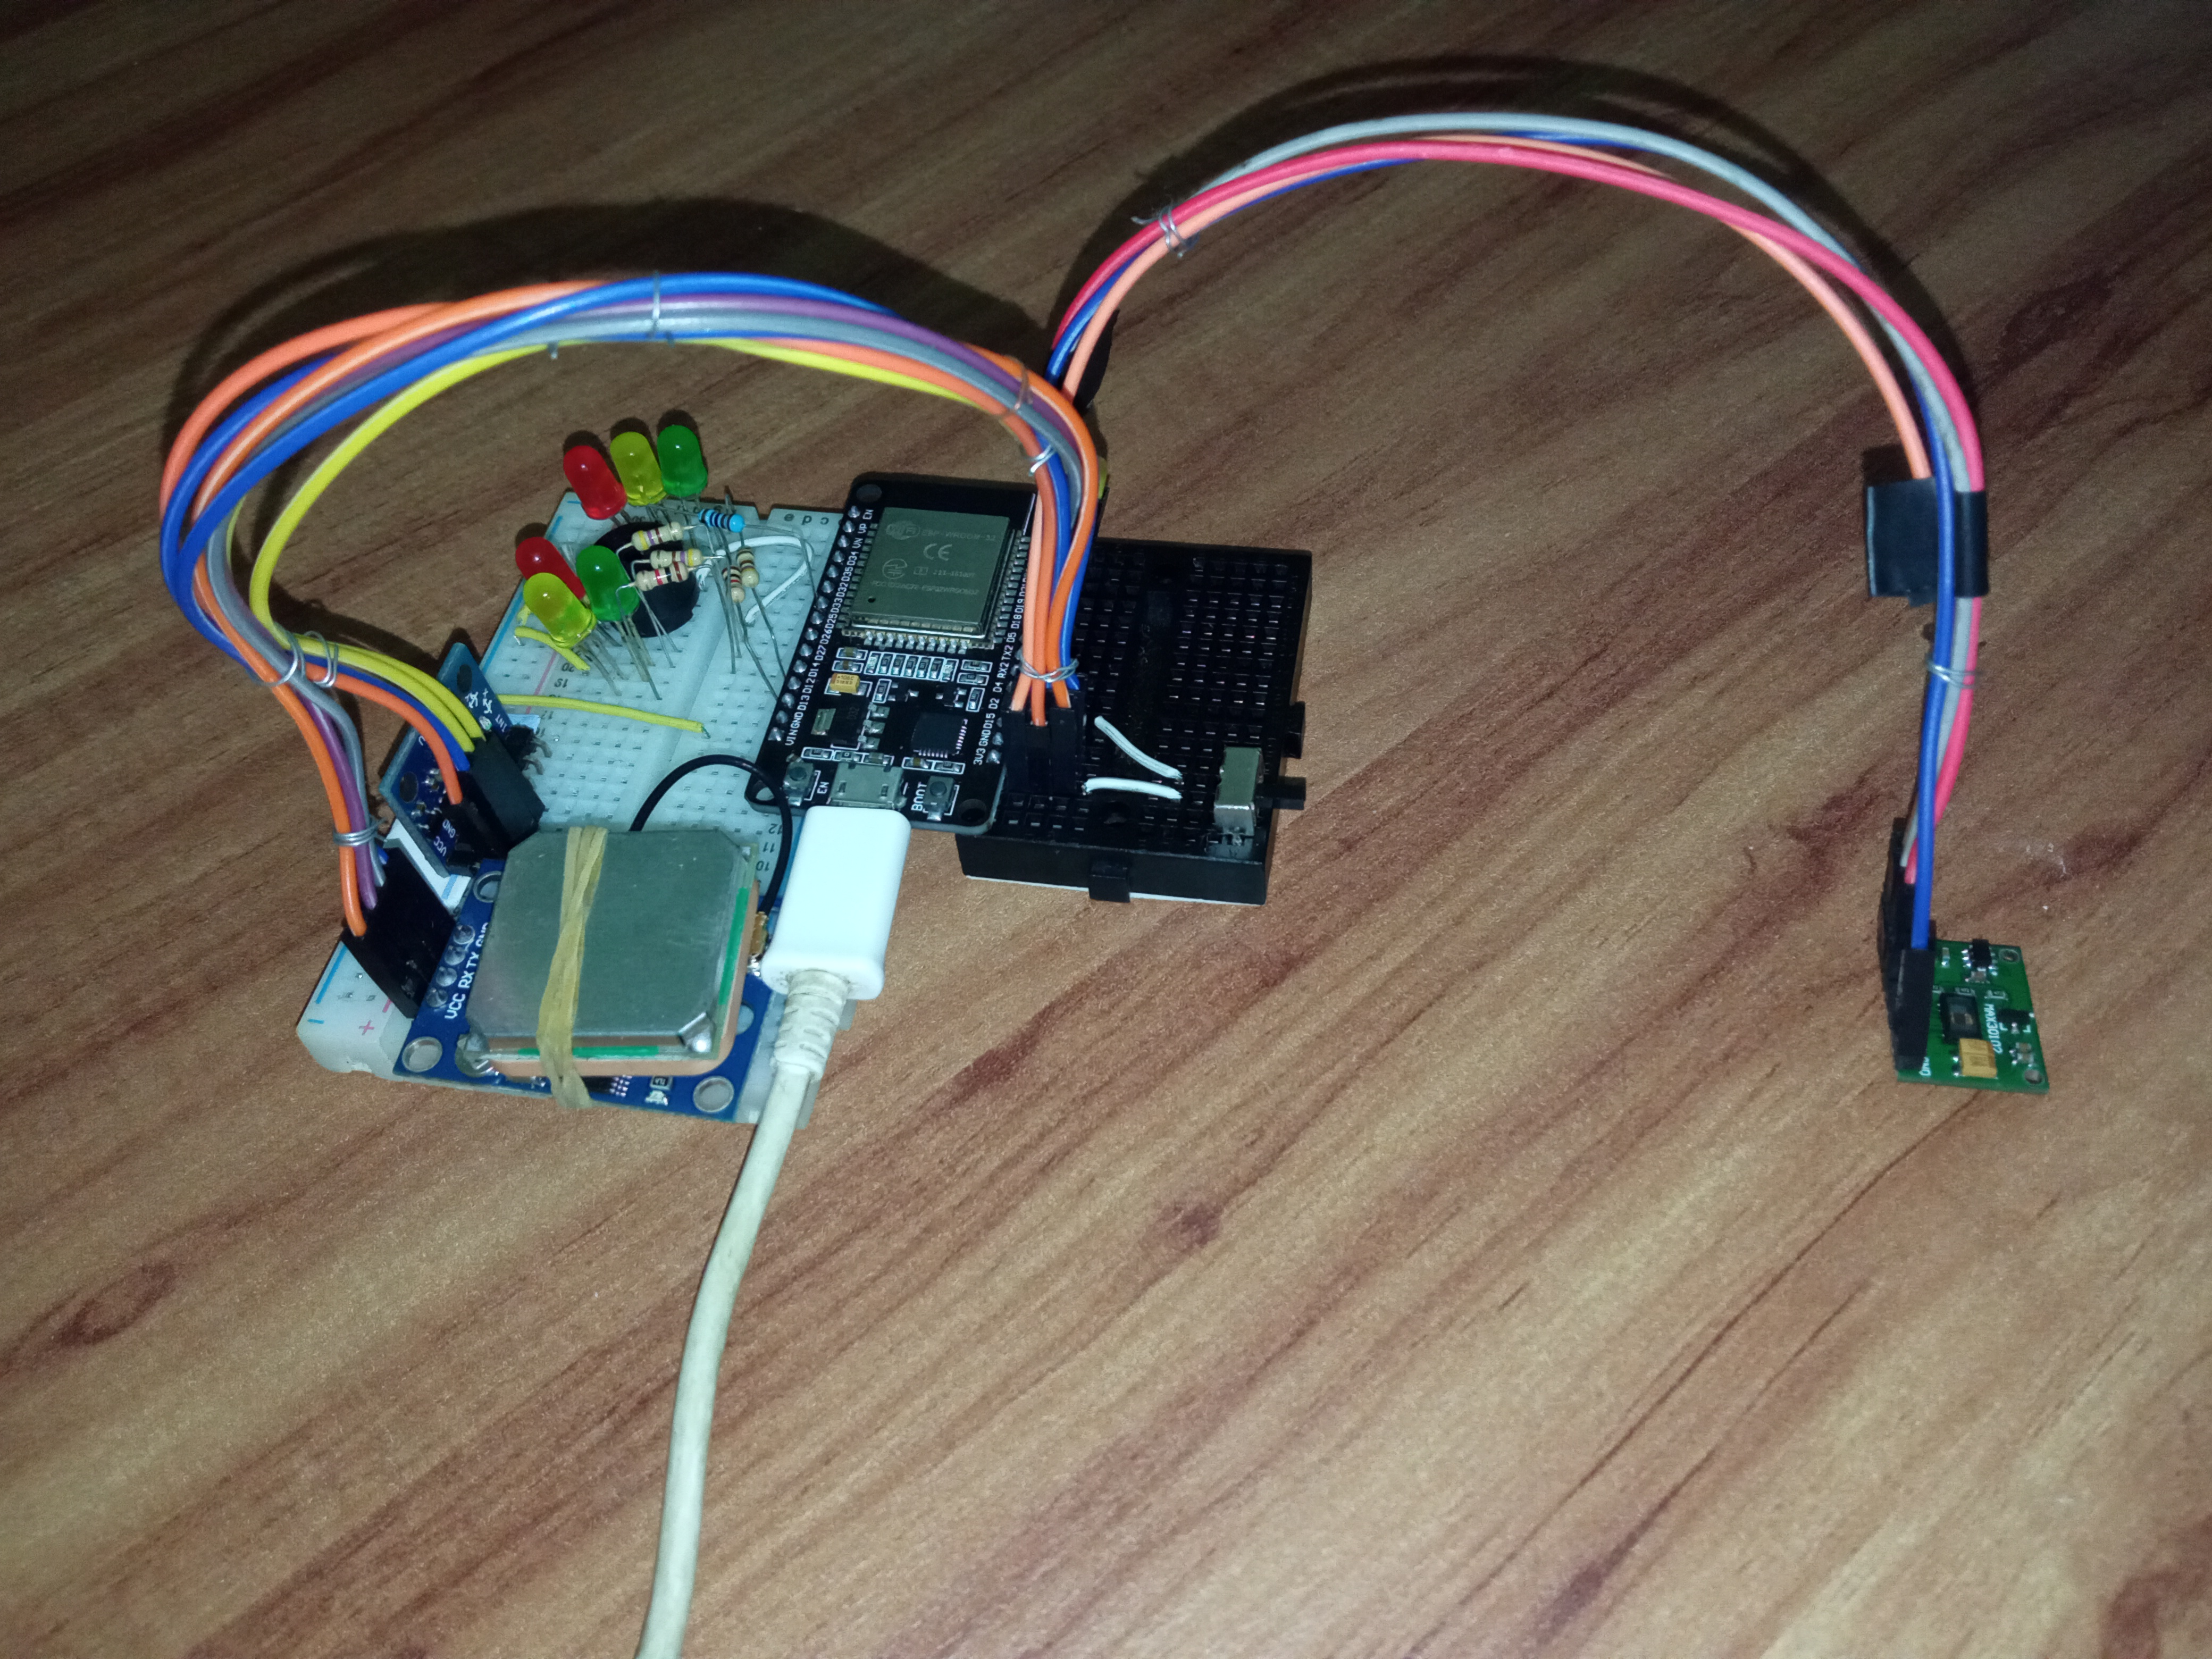
\includegraphics[width=0.7\textwidth]{figures/resultadosPrototipo/prototipo2.jpg}
    \legend{Fonte: Os autores, 2023}
    \label{fig:prototipo2}
\end{figure}

\setcounter{mpfootnote}{2}
\footnotetext[2]{Os dados apresentados se mantém irreais pois para realização da troca da imagem seria necessário o ESP32, que já foi devolvido ao professor.}

A Tabela \ref{media-dos-erro-newton} apresenta os valores das médias dos erros de OF2 e de Newton\\

\begin{table}[htb]
\centering
\ABNTEXfontereduzida
\captionsetup{justification=centering}
\caption[Médias dos erros de OF2 e Newton]{Médias dos erros de OF2 e Newton}
\label{media-dos-erro-newton}
\begin{tabular}{ |p{3cm}|p{3cm}|p{3cm}|  }
\hline
\multicolumn{3}{|c|}{Média do erro} \\
\hline
Ocupação & OF2 & Newton\\
\hline
 0 & 0.5732 & 0.6042\\
 10 & 0.7176 & 0.6010\\
 20 & 0.5065 & 0.4711\\
 30 & 0.4402 & 0.3929\\
 40 & 0.5387 & 0.5340\\
 50 & 0.5150 & 0.4740\\
\hline
\end{tabular}
\legend{Fonte: O autor, 2023}
\end{table}

	\chapter*{}
\noindent
\phantomsection{\MakeUppercase{\textbf{Conclusão e Trabalhos futuros}}}
\addcontentsline{toc}{chapter}{CONCLUSÃO E TRABALHOS FUTUROS}
\newline
\newline


O desenvolvimento deste projeto contribuiu...

Foi realizado um experimento ...

De maneira geral, o projeto alcançou com sucesso seus objetivos gerais pois conseguiu  ...

O resultado final apresentado demonstrou ...

Conclui-se que ...

Como sugestão de trabalhos futuros ....

\vspace{0.5cm}
\textit{< A conclusão proporciona um resumo sintético, mas completo, da
argumentação, das provas consignadas no desenvolvimento do trabalho,
como decorrência natural do que já foi demonstrado. Essa parte deve reunir as características do que chamamos de síntese interpretativa dos
argumentos ou dos elementos contidos no desenvolvimento do trabalho.
>}

< Mais detalhes sobre as regras de construção de uma tese, ver o documento: roteiro\_uerj\_web >

    % \include{trabalhosFuturos}

    % a abntex2-cite nao aceita o comando \nocite{*}
% portanto cada referencia nao citada deve ser
% adicionada aqui para constar na bibliografia

%\nocite{abnt-classe-doc}

% \nocite{abntex2classe}
% \nocite{abnt-bibtex-doc}
% \nocite{abnt-bibtex-alf-doc}
% \nocite{abnt-classe-doc}
% \nocite{tabela-simbolos-doc}
% \nocite{knuth}
% \nocite{lamport}
% \nocite{lrparsing}
% \nocite{intautomata}
% \nocite{inttheory}
% \nocite{contextfreel}
% \nocite{Kaltofen82factorizationof}
% \nocite{algebramoresym}
% \nocite{elementaryalg}
% \nocite{mathmethods}
% \nocite{symbc}
% \nocite{appliedaero}
% \nocite{cursocalculo}
% \nocite{languagechange}
% \nocite{structureint}
% \nocite{Bartholomew-Biggs2000ADo}
% \nocite{cidoribeiro}
% \nocite{educmat}
% \nocite{useeducation}
% \nocite{precedence}
% \nocite{intautdiff}
% \nocite{autdifftech}
% \nocite{evalderivatives}
% \nocite{modernalgebra}
% \nocite{algalgebra}

\nocite{edirlei2015}
\nocite{fischerGrodzinsky1993}
\nocite{iphoneApple}
\nocite{tiobeAbout}
\nocite{tiobeDefinition}
\nocite{stackOverflowAbout}
\nocite{stackOverflowRanking}
\nocite{qrCodeCanalTech}
\nocite{qrCodeOlharDigital}

\nocite{captchaGoogle}
\nocite{captchaG1}
\nocite{captchaExame}
\nocite{captchaTecmundo}
\nocite{captchaWikipedia}

\nocite{nfceDefinicao}

\nocite{desenvolvimentoMobile}
\nocite{xamarimDefinicao}

\nocite{nodeJsSobre}
\nocite{nodeJsMDN}
\nocite{angularIntroduction}
\nocite{angularWiki}
\nocite{vueJsAbout}
\nocite{vueJsWiki}
\nocite{reactAbout}
\nocite{reactWiki}
\nocite{reactNativeAbout}
\nocite{reactNativeWiki}

\nocite{silberschatz2016sistema}

\nocite{cheerio}
\nocite{heroku}
\nocite{githubStudentPack}
\nocite{webscrapingRockContent}
\nocite{pixDefinicao}
\nocite{mobileDatabase}
\nocite{menorPrecoApp}
\nocite{pinngoApp}
\nocite{meusPrecosApp}
\nocite{melhorPrecoAmazonasApp}

\nocite{mongoDBDefinition}
\nocite{flutterDefinition}
\nocite{beautifulSoupDefinition}
\nocite{jSoupDefinition}
\nocite{jSoupAndroid}
\nocite{expo}
\nocite{expoOverview}
\nocite{inflacaoEstadoMinas}
\nocite{inflacaoEstadao}
\nocite{blackFridayVeja}
\nocite{tiposBancoDeDados}
\nocite{sqLite}
\nocite{javascriptHistoria}
\nocite{formValidation}
\nocite{javascriptWikipedia}
    \bibliography{tcc}
	% Elementos pós-textuais
	\postextual
	% \include{glossario}

	\apendices

\chapter{A experiência de cuidar}
<OPCIONAL>\\
(INFORMAÇÃO ELABORADA PELO PRÓPRIO AUTOR DA MONOGRAFIA)

\chapter{A experiência de estudar}
OPCIONAL\\
(INFORMAÇÃO ELABORADA PELO PRÓPRIO AUTOR DA MONOGRAFIA)

	\anexos

\chapter{Estatuto da criança e do adolescente}
<OPCIONAL>\\
(INFORMAÇÃO complementar e comprobatório do texto; NÃO ELABORADA PELO AUTOR DA MONOGRAFIA)


 
	
	
	\appendix

% O algoritmo desenvolvido, na linguagem Python versão 3.7.13, está disponível no seguinte link – \textcolor{blue}{\href{https://colab.research.google.com/drive/15zD5uLvgFG42-VionRbaLIMLS6nAn-d3?usp=sharing}{Predição de casos de COVID-19 em Nova Friburgo}}  – de forma aberta, no Google Colaboratory, para fins de pesquisa e aprofundamento do estudo.
    
\end{document}
